\section{Results} \label{sec:results}
We present the posterior distributions of our DEM parameters for the SIMBA
(orange), TNG (blue), and EAGLE (green) hydro simulations in
Figure~\ref{fig:abc}. The contours mark the $68\%$ and $95\%$ confidence intervals
The posteriors are derived using ABC (Section~\ref{sec:abc}).
and describe the parameters in Section~\ref{sec:dem} and Table~\ref{tab:free_param}. 

Furthermore, we present the observables predicted by the posteriors in
Figure~\ref{fig:dem}. 
\ch{Can we construct a simple empirical model for dust that allows us to
marginalize over dust?} With the flexibility from the DEM we can reproduce observables pretty
accurately. \ch{some quantitative comparison of this?} 
\ch{What are some applications for DEMs?}
Realistic mock catalogs that reproduce observations in observable-space rather
than physical parameter space.  

Despite the significant differences in their SMFs and $M_*$-SFR relations 
(Figures~\ref{fig:smfs} and~\ref{fig:msfr}), we find a number of consistent
trends across the simulations. For instance, in all three simulations, we 
find significant positive $M_*$ dependence of $\tau_V$: $\mtaum \sim 2$. 
\ch{what does this mean?}
\ch{how does this compare to the literature?} 

We also find overall little $M_*$ and ${\rm SFR}$ dependence in the
slope offset, $\delta$, of the attenuation curve. 
\ch{what does this mean?}
\ch{how does this compare to the literature?} 
This is consistent with \cite{salim2020}, who used 23,000 galaxies with deep UV from GALEX-SDSS-WISE Legacy Catalog 2. 

paragraph on the variation of attenuation curves based on 
\ch{what does this mean?}
While an empirical prescription like DEM doesn't allow explicit modeling of the
complex dust-star geometry, it does a good job at mimicking it. 
\ch{how does this compare to the literature?} 
comparison to \cite{narayanan2018} paper 

paragraph on restating how we can learn about dust through DEMs based on trends we see
across all simulations. summarize main findings again. 

\ch{What do the differences in DEM parameters say about the differences among
the hydro sims?} 
The whole SIMBA discrepancy

\begin{figure}
\begin{center}
    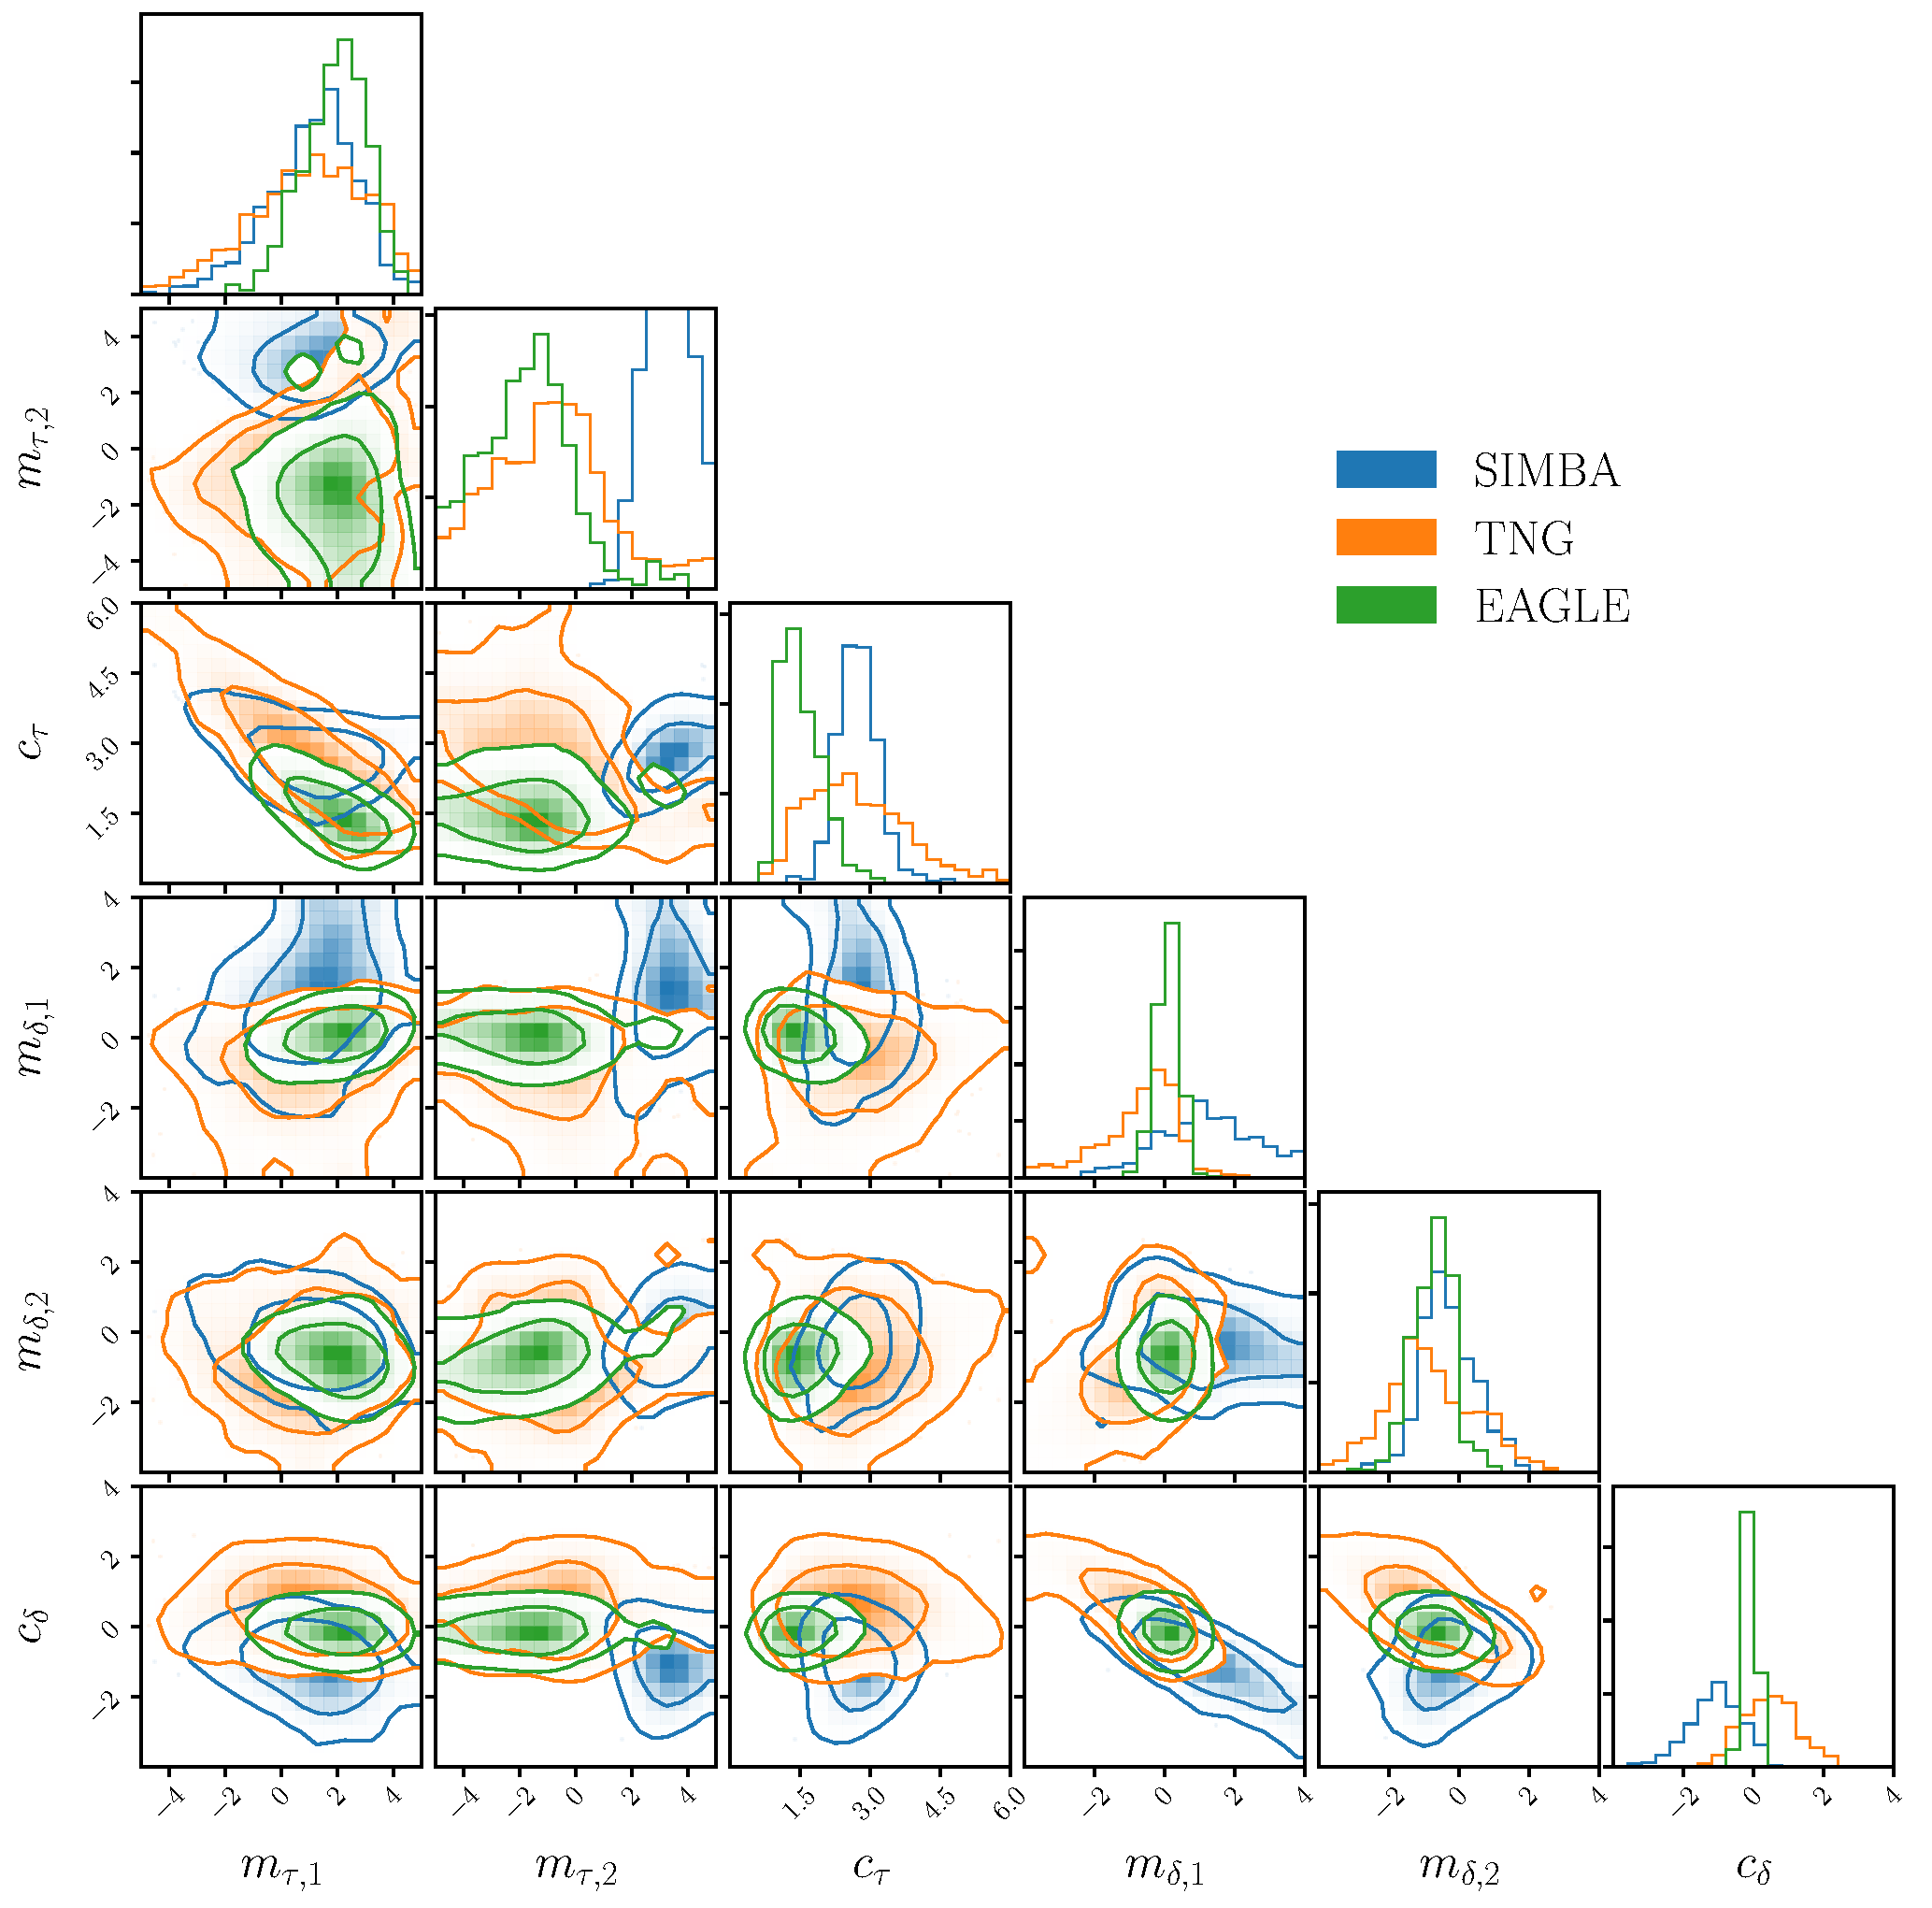
\includegraphics[width=\textwidth]{figs/abc.pdf}
    \caption{\label{fig:abc}
    Posterior distributions of our DEM parameters for the SIMBA (orange), TNG
    (blue), and EAGLE (green) hydro simulations. The contours mark the $68\%$
    and $95\%$ confidence intervals. We derive these posteriors using
    Approximate Bayesian Computation (ABC, Section~\ref{sec:abc}) and describe
    the parameters in Section~\ref{sec:dem} and Table~\ref{tab:free_param}. 
    In all simulations, dust attenuation increases for higher $M_*$ galaxies 
    ($m_{\tau,M_*} \sim 2$). The simulations also have consistent optical 
    depth amplitudes ($c_\tau$). However, the ${\rm SFR}$ dependence of
    $\tau_V$ is different among the simulations. For TNG and EAGLE,
    star-forming galaxies have lower $\tau_V$; for SIMBA quiescent galaxies
    have lower $\tau_V$. Meanwhile, for the slope offset of the attenuation
    curve, $\delta$, we find little $M_*$ and ${\rm SFR}$ dependence in the
    simulations and that the amplitude ($c_\tau$) is consistent with 0. 
    }
\end{center}
\end{figure}

\begin{figure}
\begin{center}
    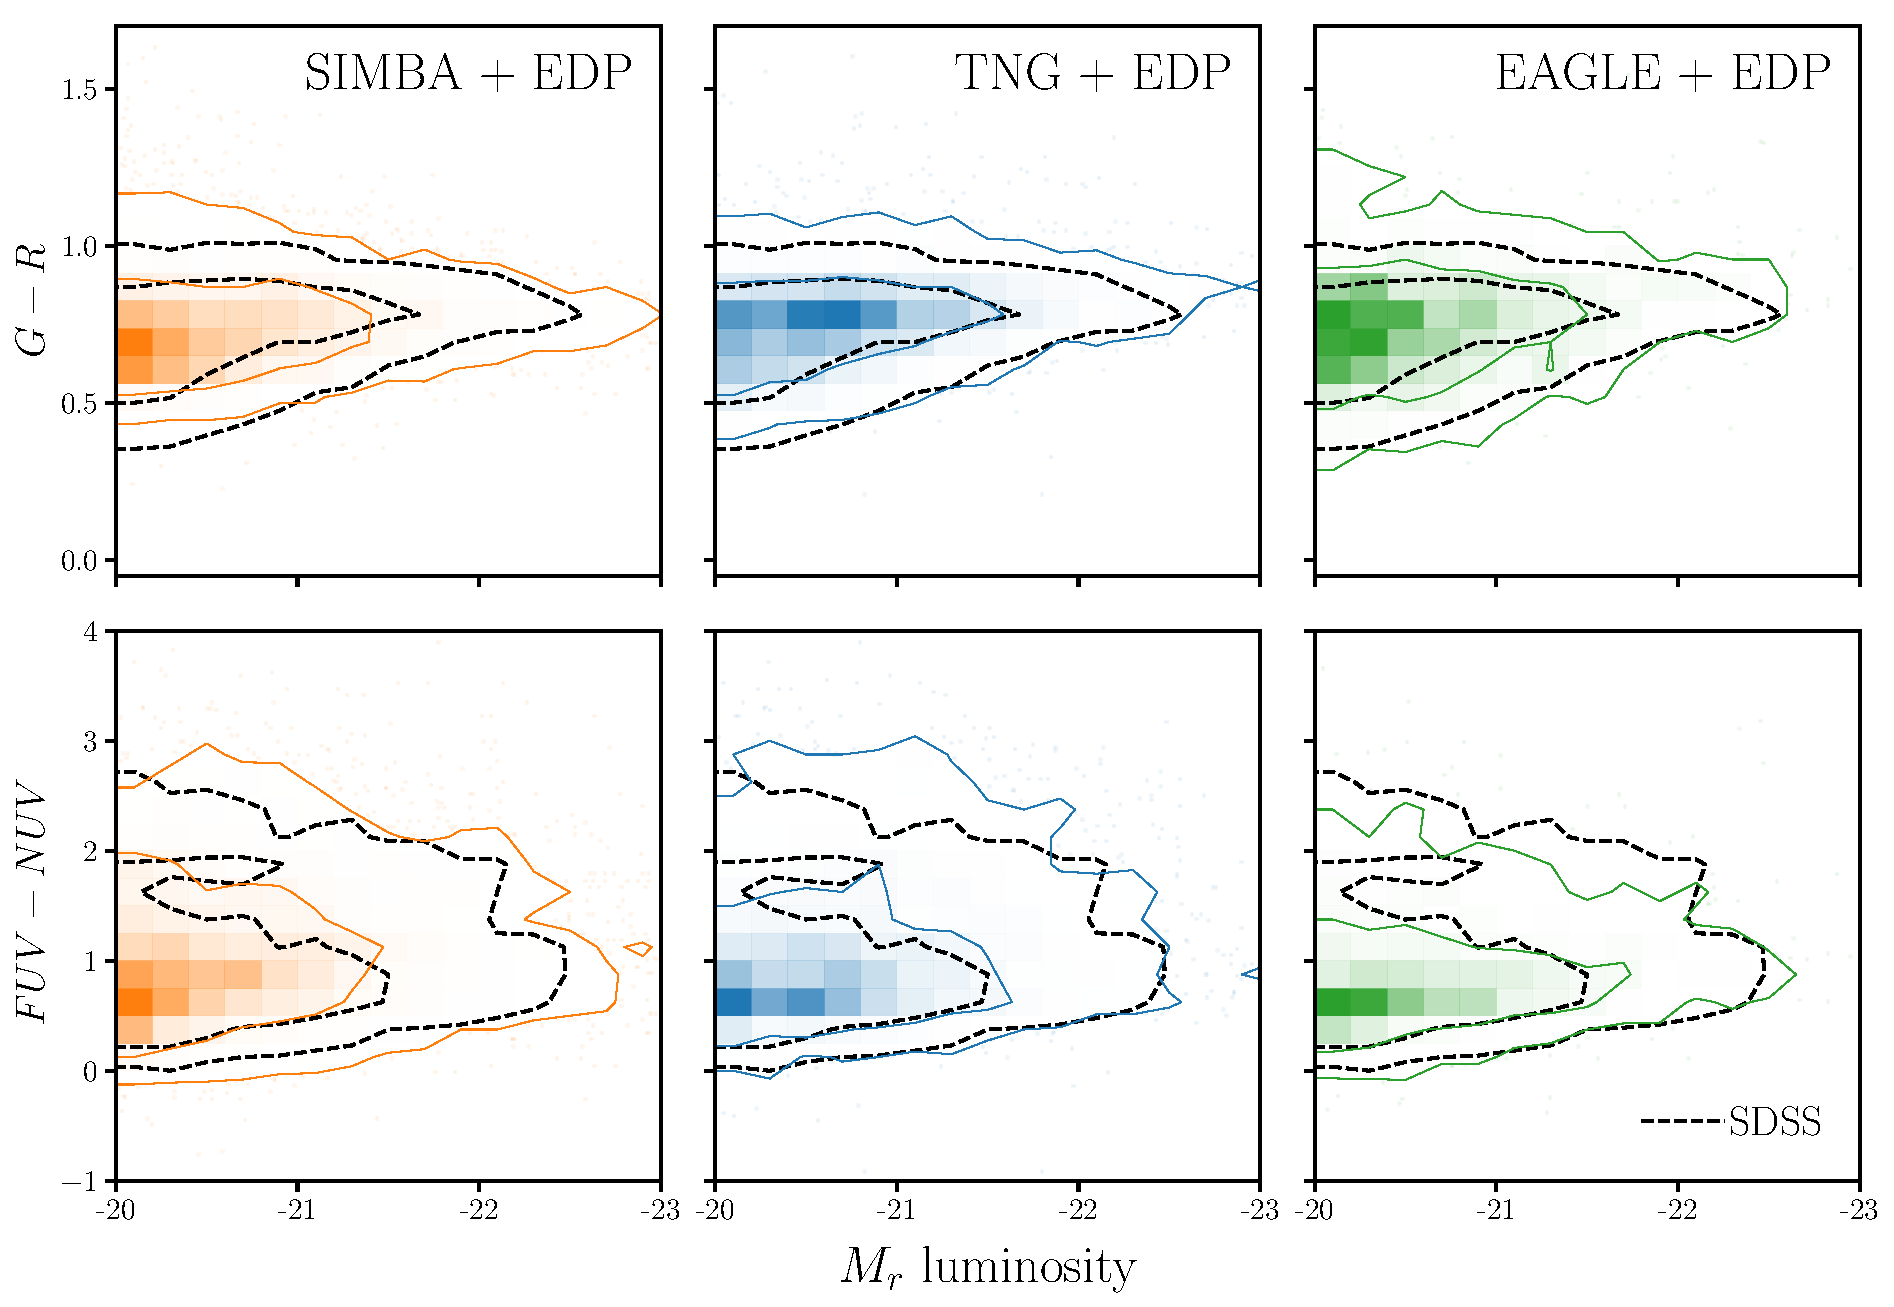
\includegraphics[width=\textwidth]{figs/abc_observables.pdf}
    \caption{Comparison of the observables predicted by the simulations with
    the posterior DEM.}
\label{fig:dem}
\end{center}
\end{figure}


What are the limitations of DEM and how can it be improved? 
\begin{itemize}
    \item too many luminous galaxies
    \item color distribution isnt' perfect. 
    \item There isn't a whole lot of flexibility for SFR=0 galaxies predicted by
    simulations and they do not agree well with observations \ref{sec:res}. 
\end{itemize}


\begin{figure}
\begin{center}
    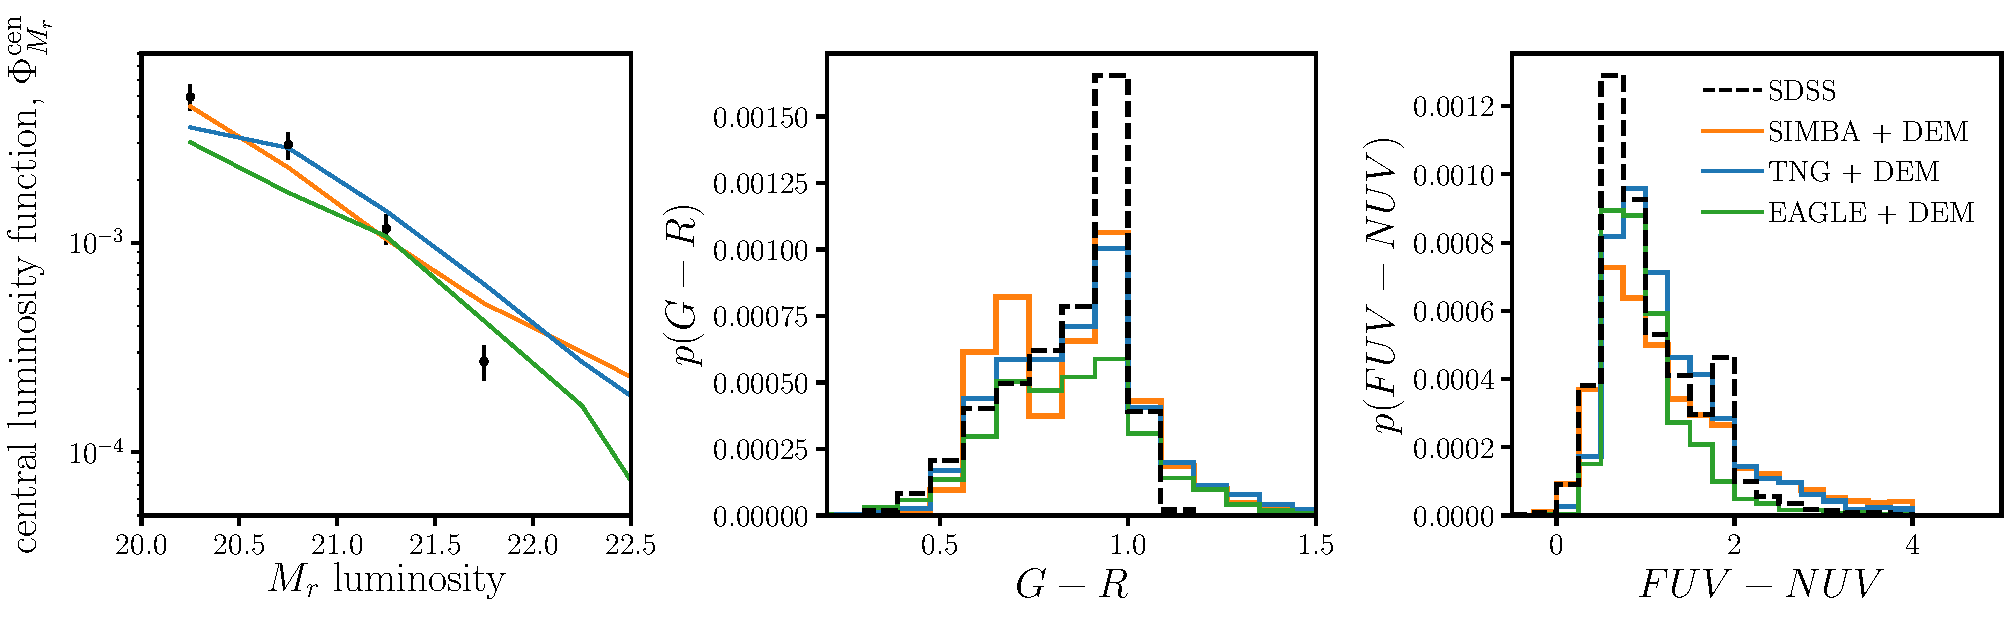
\includegraphics[width=\textwidth]{figs/abc_observables_1d.pdf}
    \caption{Comparison of the observables predicted by the simulations with
    the posterior DEM.}
\label{fig:dem1d}
\end{center}
\end{figure}




\ch{How robust are our results?}
We fix the UV bump to reduce the number of parameters. But when run our
analysis without fixing the UV bump, we find it does not impact our results.
We also get no constraints on the UV bump parameters. 

We rely on the slab model. But nothing changes when we use a more flexible
truncated normal distribution in Appendix~\ref{sec:nonslab}. tnorm DEM model allows us to also vary the
scatter of the attenuation curve 

\ch{prior?}
%\begin{figure}
%\begin{center}
%    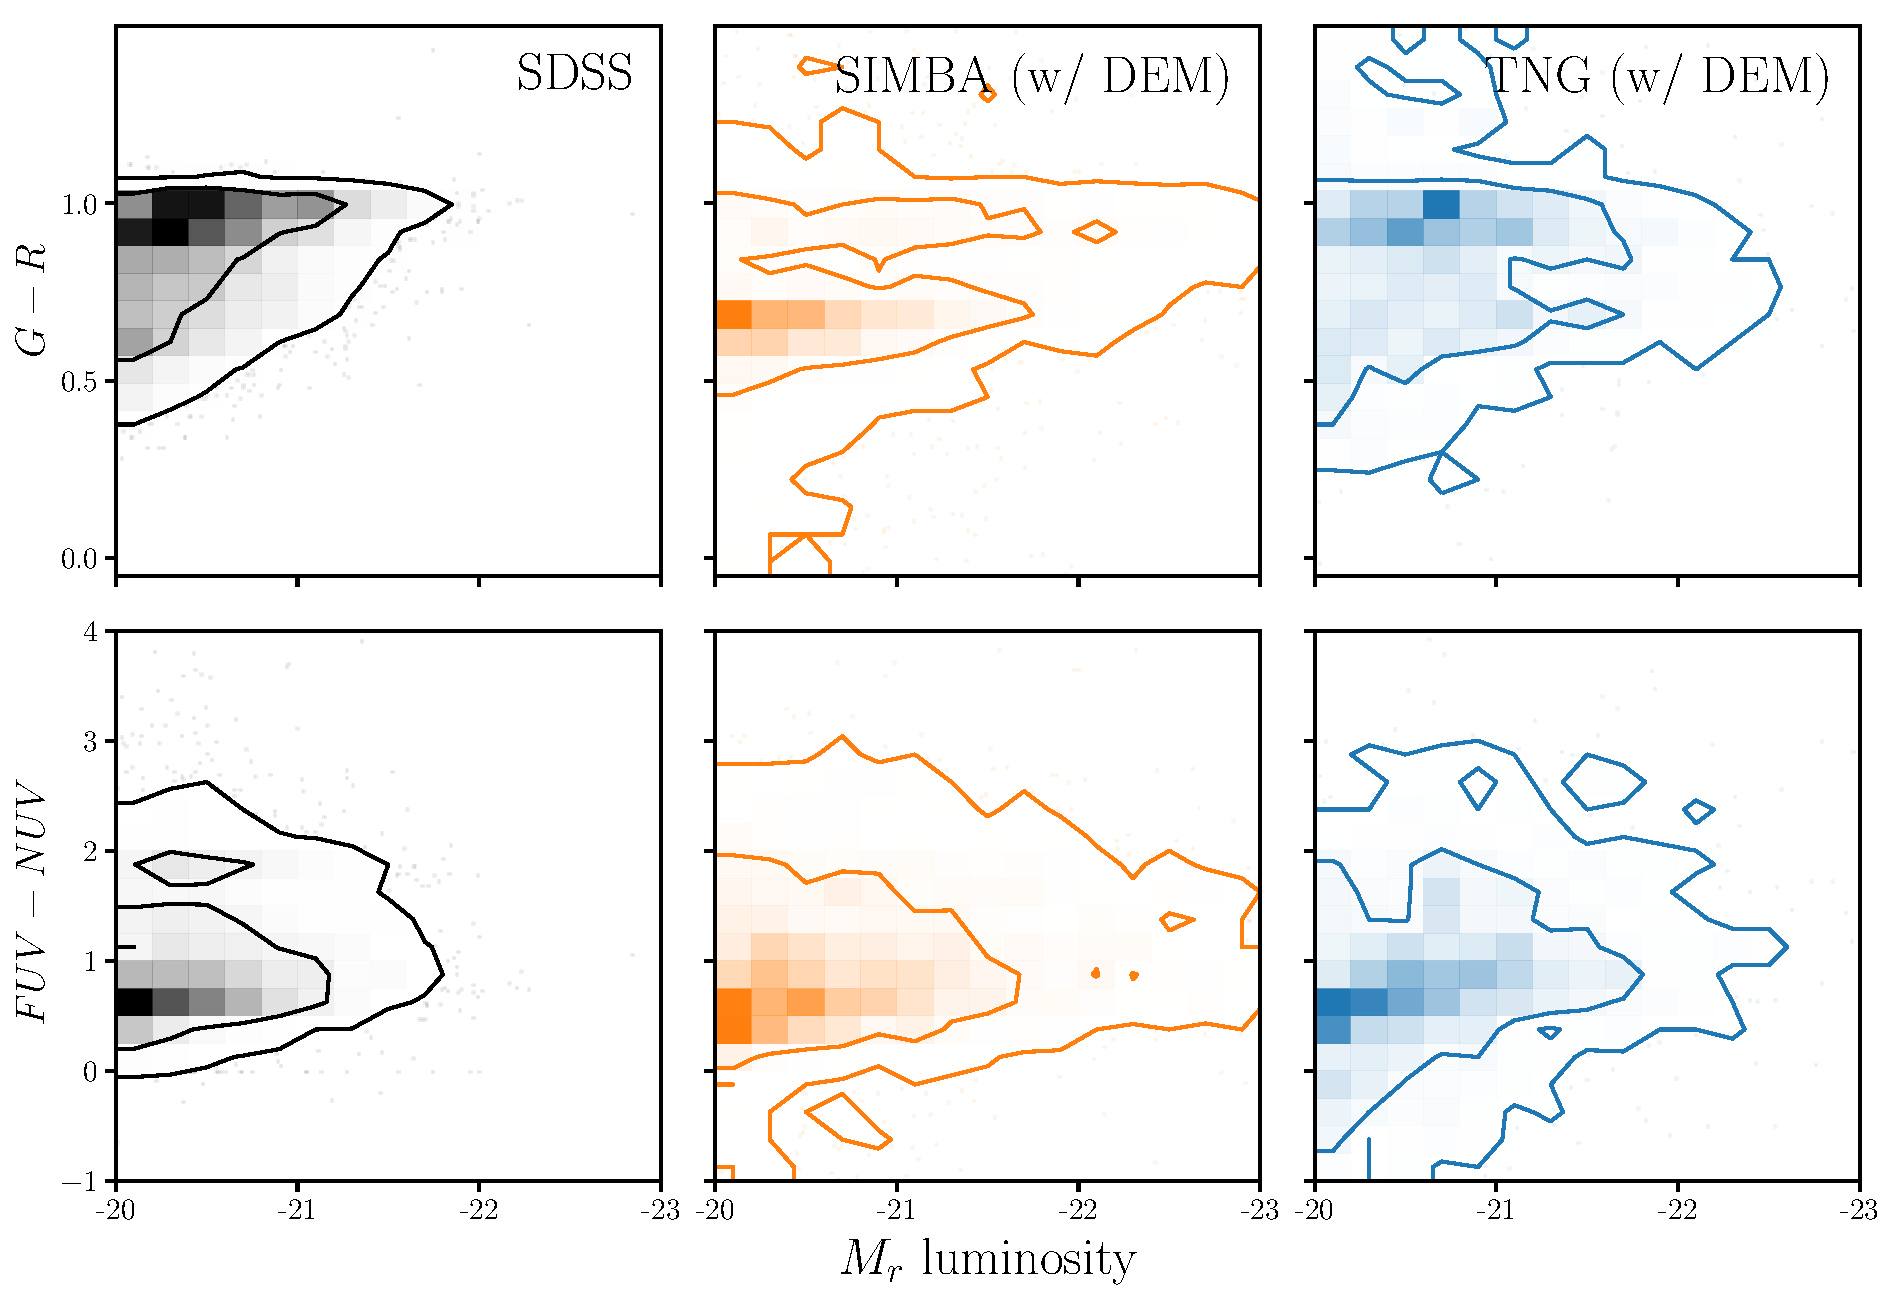
\includegraphics[width=\textwidth]{figs/abc_tnorm_observables.pdf}
%    \caption{Comparison of the observables predicted by the simulations with
%    the posterior DEM.}
%\label{fig:dem}
%\end{center}
%\end{figure}

\ch{If we marginalize over dust, can we learn anything about galaxy evolution
from the simulation?}

Are there observables that hydro sims + DEMs cannot reproduce? What does that say about the hydro sims?

What observables are unaffected by DEMs? We should chase those observables. 

We clearly have to becareful with overinterpreting hydro sims because a flexible dust model can do miracles
\begin{itemize}
    \item Should we bother calibrating our empirical and semi-analytic models
        to hydrodynamic simulations when the hydro sims also require
        marginalizing over dust parameters? Does this mean that if our goal is
        to make realistic mocks, we can be relatively careless about 
\end{itemize}
%\begin{figure}
%\begin{center}
%    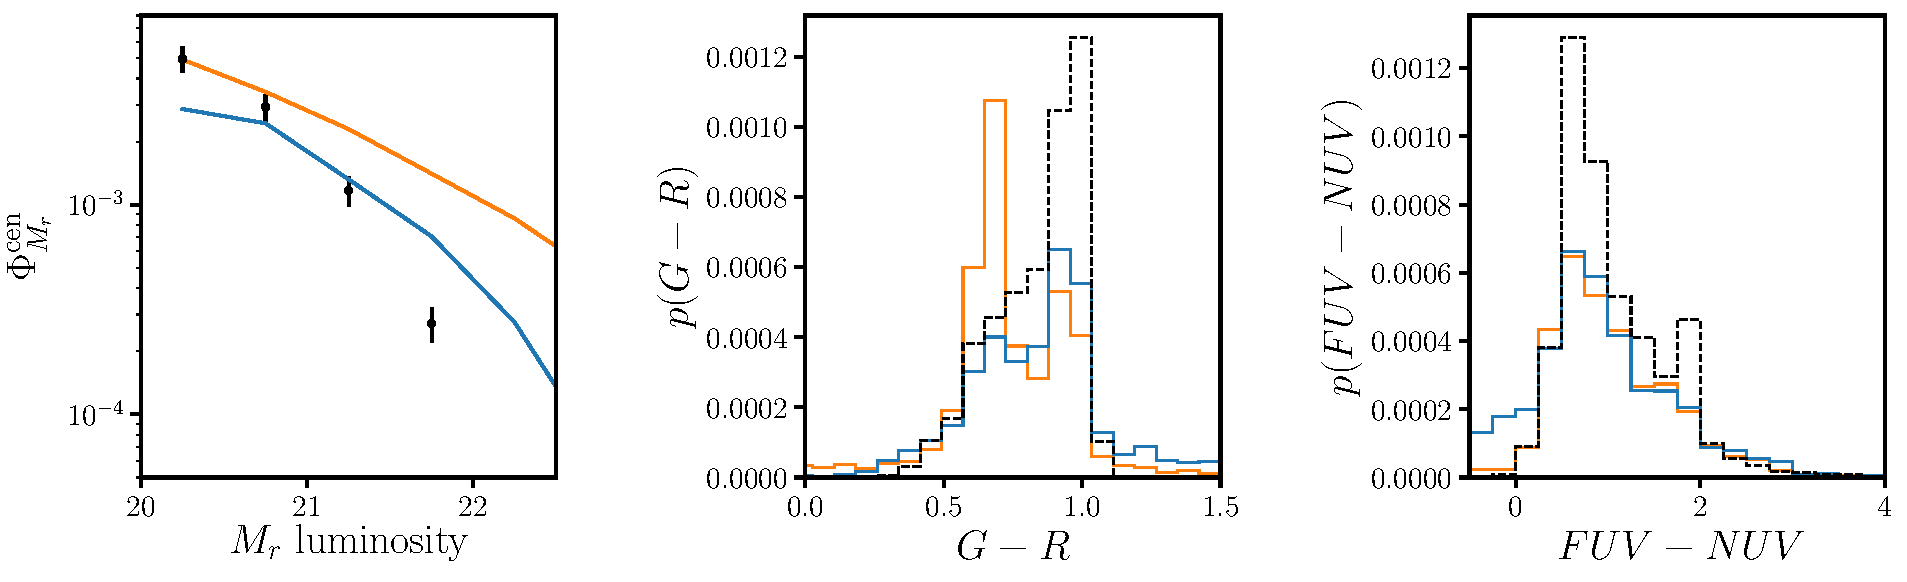
\includegraphics[width=\textwidth]{figs/abc_tnorm_observables_1d.pdf}
%    \caption{Comparison of the observables predicted by the simulations with
%    the posterior DEM.}
%\label{fig:dem}
%\end{center}
%\end{figure}
